\graphicspath{{img/chapter_1/}}

% \begin{savequote}
% ``Trying to reinvent the wheel is a lot of work. It's okay to make some tweaks and enjoy the ride." 
%     \qauthor{Karen Lamb}
% \end{savequote}

\chapter{Introduction}
\label{chapter:introduction}

% \begin{synopsis}
% Background on DM and its current status
% \end{synopsis}
%%%%%%%%%%%%%%%%%%%%%%%%%%%%%%%%%%%%%
%%%%%%%%%%%%%%%%%%%%%%%%%%%%%%%%%%%%%
%%%%%%%%%%%%%%%%%%%%%%%%%%%%%%%%%%%%%

Dark Matter is an enigma in modern physics. Despite the significant scientific
effort that has gone into trying to discern its nature, a definitive detection
proving its existence eludes us. Nevertheless, dark matter's influence 
on our Universe is undeniable, with evidence supporting its existence arising on \fixMV{all} scales, large and small.


%%%%%%%%%%%%%%%%%%%%%%%%%%%%%%%%%%%%%
%%%%%%%%%%%%%%%%%%%%%%%%%%%%%%%%%%%%%
%%%%%%%%%%%%%%%%%%%%%%%%%%%%%%%%%%%%%
\section{Evidence for Dark Matter}
%%%%%%%%%%%%%%%%%%%%%%%%%%%%%%%%%%%%%
%%%%%%%%%%%%%%%%%%%%%%%%%%%%%%%%%%%%%
%%%%%%%%%%%%%%%%%%%%%%%%%%%%%%%%%%%%%

Today, the amount of evidence in support of dark matter's existence is overwhelming. This evidence comes from astrophysical and cosmological observations inconsistent with a universe composed entirely of visible matter. This section serves as a review of this evidence. 

%%%%%%%%%%%%%%%%%%%%%%%%%%%%%%%%%%%%%
%%%%%%%%%%%%%%%%%%%%%%%%%%%%%%%%%%%%%
\subsection{Astrophysical Observations}
%%%%%%%%%%%%%%%%%%%%%%%%%%%%%%%%%%%%%
%%%%%%%%%%%%%%%%%%%%%%%%%%%%%%%%%%%%%

\subsubsection*{Galaxy Clusters}

Some of the first hints of dark matter's existence came from observations of galaxy clusters. Perhaps the most famous analysis was performed by Fritz Zwicky~\cite{Zwicky:1937zza_MassesNebulaeClusters}, who was puzzled by the high rotational velocities of galaxies within the Coma Cluster. By applying the virial theorem, equating the cluster's kinetic and gravitational potential energies, he found that the cluster would need to contain a much more significant amount of \textit{dunkle materie} (dark matter) than visible matter to accommodate these high velocities.

\subsubsection*{Rotation Curves of Spiral Galaxies}

The anomalous rotational velocities observed in galaxy clusters can also be observed at the galactic scale. The rotation curves of spiral galaxies, which relate the rotational velocities of stars to their distance from the galactic centre, were observed to be flat at large distances. From the observed distribution of visible matter, Newtonian mechanics predicts that the orbital velocity of a star a distance $r$ from the galactic centre, $v_\star(r)$, is related to the mass of the galaxy, $M(r)$, through
\begin{equation}
    v_\star(r) = \sqrt{\frac{G M(r)}{r}},
\end{equation}
indicating that the velocity should fall off as $1/\sqrt{r}$ at the outer regions of the galaxy where $M(r)$ is constant. Instead, observations of many spiral galaxies indicate that this velocity remains constant out to the galaxy's edge. 

A simple way to produce such a rotation curve is to introduce a spherically symmetric distribution of dark matter around the galaxy,
\begin{equation}
    \rho_{\mathrm{DM}}(r) = \frac{v_0^2}{4 \pi G r^2},
\end{equation}
that results in a constant rotational velocity of $v_0$ out to the galaxy edge. Detailed simulations of structure formation in a Cold Dark Matter (CDM) Universe indicate that the dark matter halo follows a Navaro-Frenk-White (NFW) profile, \fixMV{cite for NFW}
\begin{equation}
    \rho_{\mathrm{DM}}(r) = \frac{\rho_0}{\left( \frac{r}{r_\mathrm{s}}\right)\left( 1 + \frac{r}{r_\mathrm{s}}\right)^2},
\end{equation}
where $\rho_0$ and $r_\mathrm{s}$ are free parameters that must be fit to each halo. 
% More detailed simulations show that the true profile deviates slightly from an NFW, instead being more appropriately modelled by an Einasto profile. However, both profiles are observationally indistinguishable.

An example rotation curve for galaxy NGC 6503 is presented in Fig.~\ref{fig:gal_rotn_curve}, with the contributions from each of the matter components to the rotational velocity shown~\cite{Freese:2008cz_may_ReviewObservationalEvidence, Lelli:2016zqa_SPARCMassModels}. As can be seen, the visible matter constituting disk and gas components does not explain the observed rotational velocity. 

\begin{figure}[t!]
    \centering
    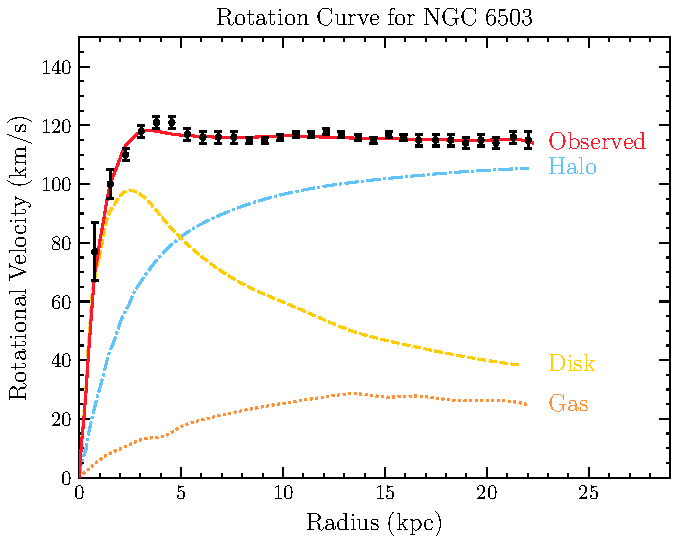
\includegraphics{gal_rotn_N6503}
    \caption{Galaxy rotation curve for NGC 6503, showing the contributions to the total velocity (red) from the DM halo (blue), disk (yellow), and gas components. Data used in making this plot was obtained from~\cite{Freese:2008cz_may_ReviewObservationalEvidence, Lelli:2016zqa_SPARCMassModels}.}
    \label{fig:gal_rotn_curve}
\end{figure}

\subsubsection*{Gravitational Lensing}

As General Relativity describes, the curvature of space-time around massive entities causes light to travel along curved paths. As such, the mass of astrophysical structures can be deduced from the extent to which objects in the background are gravitationally lensed. The disparity between the mass obtained from gravitational lensing and the mass of visible matter in the system is further evidence of dark matter's existence. 

\subsubsection*{The Bullet Cluster}

The bullet cluster is the result of two colliding galaxy clusters which the Chandra X-ray telescope imaged. When viewed in the X-ray, the smearing of the visible matter after the collision is clearly seen, as shown in the red regions of Fig.~\ref{fig:bullet_cluster}, which is expected from such a collision. However, when the gravitational potential was mapped using gravitational lensing, it was clear that the majority of the mass was displaced relative to the visible matter. This mass is attributed to the dark matter components of the original clusters. As indicated by the purple regions in Fig.~\ref{fig:bullet_cluster}, the dark matter halos seem to have passed through each other mostly unperturbed. This tells us that not only is the majority of the mass comprised of dark matter, but that the dark matter has extremely small interactions with both the visible matter and itself. 

\begin{figure}[t!]
    \centering
    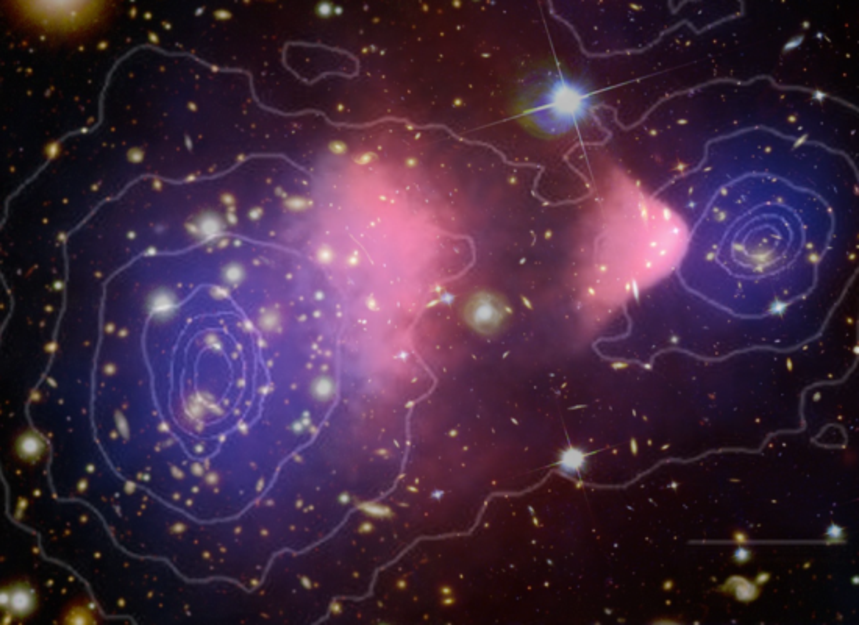
\includegraphics[width = 0.75\textwidth]{bullet_cluster}
    \caption{Image of the Bullet Cluster with contours of the gravitational potential superposed. The red regions indicate the baryonic matter after the collision, while the purple regions are the expected DM components deduced from gravitational lensing. \fixMV{cite}}
    \label{fig:bullet_cluster}
\end{figure}

%%%%%%%%%%%%%%%%%%%%%%%%%%%%%%%%%%%%%
%%%%%%%%%%%%%%%%%%%%%%%%%%%%%%%%%%%%%
\subsection{Cosmological Evidence}
%%%%%%%%%%%%%%%%%%%%%%%%%%%%%%%%%%%%%
%%%%%%%%%%%%%%%%%%%%%%%%%%%%%%%%%%%%%

Dark matter has played a major role in the cosmological history of our Universe. The current best cosmological model is the $\Lambda$-Cold Dark Matter model ($\Lambda$CDM), in which cold (i.e. non-relativistic) dark matter plays a prominent role. The relative amount of dark matter present in our Universe can be determined with measurements of the light element abundances produced via Big Bang Nucleosynthesis (BBN).

\subsubsection*{The Cosmic Microwave Background}
One of the best probes of cosmological models is the Cosmic Microwave Background (CMB). The CMB is the radiation that was emitted during recombination when the Universe had cooled enough for electrons and protons to combine and not be ionised by the photon bath. While the CMB temperature looks isotropic on large scales, fluctuations around the average value of $T_\mathrm{CMB} \sim 2.73\K$ are observed at very small scales. 
These anisotropies are the result of oscillations in the baryonic matter known as Baryon Acoustic Oscillations (BAO). These oscillations were produced due to the interplay between the outward pressure caused by matter interactions and the pull of gravitation due to dark matter. 

Measuring the angular power spectra of these anisotropies and fitting the cosmological parameters of the $\Lambda$CDM model tell us how the Universe's energy density ($\Omega_\mathrm{total}$), is partitioned between the matter ($\Omega_\mathrm{m}$), radiation  ($\Omega_\mathrm{rad}$), and dark energy  ($\Omega_\Lambda$) components. In a flat universe, of which we believe ours to be, these components should sum to $\Omega_\mathrm{tot} = 1$.
The Planck collaboration most recently performed a precise measurement of the CMB power spectrum in 2018, obtaining best-fit parameters
\begin{equation}
    \Omega_\mathrm{m} = 0.311 \pm 0.006,\quad \Omega_\Lambda = 0.689 \pm 0.006.
\end{equation}

Combining the predicted baryon density from BBN with the CMB observations breaks down the matter abundance into the dark ($\Omega_\mathrm{DM}$)  and baryonic ($\Omega_\mathrm{b}$) components yielding
\begin{equation}
    \Omega_\mathrm{DM}h^2 = 0.1193 \pm 0.0009,\quad \Omega_\mathrm{DM}h^2 = 0.02242 \pm 0.00014,
\end{equation}
where $h$ is the dimensionless Hubble constant such that the Hubble parameter today is $H_0 = 100\, h\km\s^{-1}\;\mathrm{Mpc}$. 

\subsubsection*{Large Scale Structure}
After recombination, the pressure on the baryonic matter from photons subsided, allowing the small density perturbations to grow. This would lead to the growth of stars, galaxies and the large scale structure we observe today~\cite{Springel:2006vs_LargescalestructureUniverse}. N-body simulations of the Universe's evolution require a cold dark matter component for this structure to form. While a small component of the dark matter can be warm, hot dark matter would wash out small scale structures~\cite{Springel:2005nw_Simulatingjointevolution}.  

%%%%%%%%%%%%%%%%%%%%%%%%%%%%%%%%%%%%%
%%%%%%%%%%%%%%%%%%%%%%%%%%%%%%%%%%%%%
%%%%%%%%%%%%%%%%%%%%%%%%%%%%%%%%%%%%%
\section{Potential Models of Dark Matter}
%%%%%%%%%%%%%%%%%%%%%%%%%%%%%%%%%%%%%
%%%%%%%%%%%%%%%%%%%%%%%%%%%%%%%%%%%%%
%%%%%%%%%%%%%%%%%%%%%%%%%%%%%%%%%%%%%

The general consensus amongst physicists is that dark matter has a particle nature, similar to the visible matter of the Standard Model. Models may be as simple as dark matter being described by a single field or there could be an extensive hidden sector with complicated symmetry structures. Given the few details we know about dark matter, there exists an enormous library of models that can produce a viable dark matter candidate. However, there are generic properties a good dark matter candidate must satisfy, namely:
\begin{itemize}
    \item \textbf{Stable on Cosmological Timescales:} Dark matter must either be stable or have a lifetime significantly longer than the age of the Universe in order to be present in its current abundance. 
    
    \item \textbf{Neutral or milli-charged under Electromagnetism:} Dark matter, as its name suggests, does not significantly interact with light. By requiring that dark matter be completely decoupled from the Standard Model plasma by the time of recombination yields an upper bound on the milli-charge dark matter can carry of~\cite{McDermott:2010pa_TurningLightsHow} 
    \begin{equation}
        q_\mathrm{DM}/e < \begin{cases}
            3.5\times10^{-7} \left( \frac{m_\mathrm{DM}}{1\GeV}\right)^{0.58},\quad m_\mathrm{DM} > 1\GeV\\
            4.0\times 10^{-7}\left( \frac{m_\mathrm{DM}}{1\GeV}\right)^{0.35},\quad m_\mathrm{DM} <1\GeV,
        \end{cases}
    \end{equation}
    
    \item \textbf{Small Self-Interactions:} The standard $\Lambda$CDM cosmology assumes that the dark matter is collisionless. However, small dark matter self-interactions can help resolve existing small-scale structure issues~\cite{Tulin:2017ara_feb_DarkMatterSelfinteractionsTulin:2017ara_feb_DarkMatterSelfinteractions, Spergel:1999mh_Observationalevidenceselfinteracting}. Current limits on the self-interaction cross section are $\sigma_{\mathrm{DM-DM}}/m_\mathrm{DM} < 0.48\cm^2/\mathrm{g}$ come from merging galaxy clusters~\cite{Randall:2008ppe_ConstraintsSelfInteractionCrossSection} and the ellipticity of galaxies obtained from X-ray observations~\cite{Buote:2002wd_ChandraEvidenceFlattened}.
\end{itemize}
A selection of the more prominent dark matter candidates is shown in Fig.~\ref{fig:DM_models_landscape}. The key features of a few of these models are discussed below.

\begin{figure}[t!]
    \centering
    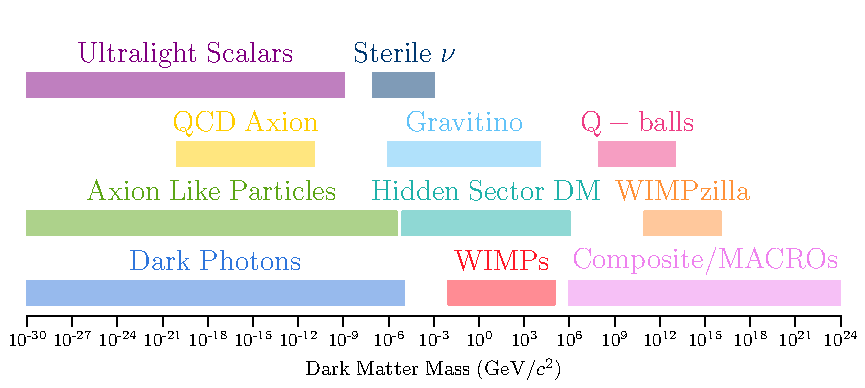
\includegraphics{DM_model_landscape}
    \caption{Illustrative landscape of dark matter models and the mass range for which they predict a valid candidate.}
    \label{fig:DM_models_landscape}
\end{figure}

\subsubsection*{WIMPs}
The Weakly Interacting Massive Particle (WIMP) is perhaps the most well-known dark matter candidate. WIMPs rose to fame thanks to the so-called ``WIMP miracle"~\cite{Feng:2010gw_DarkMatterCandidates}. This refers to the fact that particles with weak scale masses and annihilation cross sections just so happen to have the correct relic abundance of dark matter when produced via the freeze-out mechanism~\cite{Jungman:1995df_Supersymmetricdarkmatter}. In this scenario, the final WIMP abundance depends on the total annihilation cross-section, $\langle\sigma v\rangle$, with only a very mild dependence on the DM mass~\cite{Steigman:2012nb}, 
\begin{equation}
    \Omega_{\mathrm{DM}}h^2 \sim 0.12 \; \left(\frac{2.2\times 10^{-26}\cm^3 \s^{-1}}{\langle \sigma v\rangle}\right).
\end{equation}

The canonical weak-scale WIMP has been tightly constrained from direct and indirect detection limits, leading it to be disfavoured as a dark matter candidate. The term ``WIMP"  is now typically used to refer to any particle dark matter candidate that is produced thermally in the early Universe. Such a particle can have a mass in the range $10\MeV\lesssim m_\mathrm{WIMP} \gtrsim 100\TeV$. Lighter WIMPs will have non-negligible contributions to the effective number of neutrino species, $N_{eff}$, which is constrained through BBN and the Cosmic Microwave Background CMB to be $N_{eff} = 2.99 \pm 0.17$~\cite{Planck:2018vyg_sep_Planck2018results}. Masses larger than $\sim 100\TeV$ are excluded from partial wave unitarity~\cite{Griest:1989wd_UnitarityLimitsMass}. 

\subsubsection{Axions}

The original axion was proposed by by Peccei and Quinn~\cite{Peccei:1977hh_CPConservationPresence} as part of a dynamical solution to the ``Strong CP Problem". This refers to the measured value of the neutron electric dipole moment (nEDM) being anomalously small, with a current upper bound of $|d_n| < 0.18\times 10^{-26}\;e\cm$~\cite{Abel:2020pzs_feb_MeasurementPermanentElectric}. This can be translated to an upper bound on the CP-violating QCD $\theta$-parameter such that $|\theta_{QCD}|\lesssim 10^{-10}$, raising questions as to why this value seems to be fine-tuned to such a small value. 

The Peccei-Quinn solution to this problem introduces a new, anomalous, global  $U(1)_{\mathrm{PQ}}$ symmetry and promotes $\theta_\mathrm{QCD}$ to be a dynamical field.
The axion emerges as the pseudo-Goldstone boson associated with the breaking of $U(1)_\mathrm{PQ}$, such is in the two most prominent UV completions of the axion, the KSVZ~\cite{Kim:1979if_WeakInteractionSinglet, Shifman:1979if_CanConfinementEnsure} and DFSZ~\cite{_PossibleSuppressionAxion, Dine:1981rt_SimpleSolutionStrong} models. In these models, the axion produced in the early Universe can serve the role of cold dark matter today. This makes it a very compelling dark matter candidate, as it solves two of the biggest mysteries of physics in one neat package. 

However, solving the Strong CP problem can be rather restrictive on the model parameters. For example, the QCD axion's coupling to the photon is not a free parameter and depends on the scale at which the PQ symmetry is broken. Many models introduce a light pseudoscalar particle that is not associated with a solution to the Strong CP problem but has a coupling to the photon that takes the same form as the QCD axion. Such pseudoscalars are known as ``Axion Like Particles" (ALPs) and can similarly make a good dark matter candidate.

\commMV{Add some more candidates}

%%%%%%%%%%%%%%%%%%%%%%%%%%%%%%%%%%%%%
%%%%%%%%%%%%%%%%%%%%%%%%%%%%%%%%%%%%%
\subsection{Dark Matter in an Effective Fields Theory Framework}
\label{subsec:DM_EFTs}
%%%%%%%%%%%%%%%%%%%%%%%%%%%%%%%%%%%%%
%%%%%%%%%%%%%%%%%%%%%%%%%%%%%%%%%%%%%

\subsection{Overview of Effective Field Theory}
Given the sheer quantity of potential dark matter models and candidates, a model-independent approach for analysing experimental results is often desired. An economical analysis method is to use an Effective Field Theory (EFT) to describe the dark matter-Standard Model interactions. Effective theories are prevalent in all of physics, e.g., describing light using ray optics vs Maxwell's equations or the orbits of planets using Newtonian gravity vs General relativity. The delineating factor in choosing a formalism is the scale (energy, length, etc.) we are interested in. 
\commMV{Add in the usual EFT diagram}
Experiments will only be sensitive to interactions that can occur below some energy scale, i.e. $13.6\TeV$ at the LHC or $~1\GeV$ in direct detection experiments; we are only interested in describing the interactions that occur below this scale.

One follows two main schools of thought when constructing an EFT. First, there is the \textit{top down} approach. Here, you begin with a particular complete model in mind that consists of heavy and light fields. At energies below the production threshold of the heavy fields, these degrees of freedom can be ``integrated out" of the theory. This process leaves an effective theory for the interactions among the light fields. The interactions that would be mediated by the heavy fields appear as non-renormalisable operators that are suppressed by this high energy scale, $\Lambda$. 

The second method, known as the \textit{bottom-up} approach, is more agnostic to the high-energy physics that might be in play. In this method, one constructs all possible operators that obey the required symmetries of the theory up to a desired mass dimension. Operators of mass dimension greater than four are then suppressed by powers the required number of powers of the high energy cutoff scale, $\Lambda$. This cutoff scale indicates the energy at which the EFT begins to break down and should at least be larger than the masses of the fields in the EFT. The Lagrangian constructed in this manner is made out of a tower of operators, $\mathcal{O}_i^{(n)}$, forming
\begin{equation}
    \mathcal{L}_\mathrm{EFT} \supset \sum_{n>4}   \sum_{i = 1}^{j_n} \frac{C_i^{(n)}}{\Lambda^{n-4}}\mathcal{O}_i^{(n)},
\end{equation}
where we sum over all $j_n$ operators present at mass dimension $n$. The $C_i^{(n)}$ are called Wilson coefficients and are typically energy dependent.


In the context of dark matter, there are many EFTs describing the interaction at various energy scales. For example, dark matter scatting off nuclei in direct detection experiments is described by a non-relativistic EFT built out of the momentum transfer, relative velocity and spin operators of the dark matter and targets~\cite{Cirelli:2013ufw_oct_Toolsmodelindependentbounds, Fitzpatrick:2012ix_EffectiveFieldTheory}. At higher energy scales where relativistic effects become important, the EFT is instead constructed from relativistic fields, such as dark matter that may be produced in colliders.

Generally, an EFT will have fewer free parameters than the underlying UV theories, typically the dark matter mass and the high energy cutoff scale. This is in contrast with the dozens or so parameters often present in complete models. This allows for a simpler interpretation of experimental results as you will be fitting to a lower dimensional parameter space. 

\commMV{Move the next sections later?}
\subsection{Dimension 6 EFT Operators for Dirac Fermion Dark Matter}
This work's approach will focus on dimension 6 EFT operators that describe the interactions of Dirac fermion dark matter with standard model fermions. These operators will have a structure 
\begin{equation}
    \mathcal{L}_\mathrm{EFT}^{(6)} \sim \frac{1}{\Lambda^2}(\bar{\chi}\Gamma_\chi \chi)(\bar{f}\Gamma_{\mathrm{SM}}f),
\end{equation}
where the $\Gamma_i$ determines the Lorentz structure of the interaction by taking appropriate combinations from the set
\begin{equation}
    \Gamma_i\in \{1, i\gamma_5, \gamma^\mu, i\gamma^\mu \gamma^5, \sigma^{\mu\nu}, i\gamma^5 \sigma^{\mu\nu}\}.
\end{equation}
For example, the case of $\Gamma_\chi = \Gamma_\mathrm{SM} = 1$ yields scalar currents for both the DM and SM fermions and would correspond to integrating out a heavy scalar mediator in the UV theory. There are 10 such operators at dimension six that form a linearly independent basis. These are given in Table~\ref{tab:opers_defn_full}, along with spin-averaged squared matrix element for dark matter scattering with a fermion. The coupling constants, $g_f$, are given in terms of the fermion Yukawa couplings, $y_f$, and the EFT cutoff scale, $\Lambda_f$. Hence, these operators describe interactions between dark matter and the elementary fermions of the Standard Model: the leptons and quarks. 




\begin{table}[t!]
\centering
\setlength{\tabcolsep}{0.25em}   
\begin{tabular}{  c  c  c  c  c }
\toprule
  Name & Operator & $g_f$  & $|\overline{M}(s,t,m_i)|^2$   \\\midrule\midrule
  D1 & $\bar\chi  \chi\;\bar f  f $ & $\frac{y_f}{\Lambda_f^2}$  & $ g_f^2\frac{\left(4 m_{\chi }^2-t\right) \left(4 m_{\chi }^2-\mu ^2   t\right)}{\mu ^2}$ \\  
  D2 & $\bar\chi \gamma^5 \chi\;\bar f f $ & $i\frac{y_f}{\Lambda_f^2}$ & $g_f^2\frac{t \left(\mu ^2 t-4 m_{\chi }^2\right)}{\mu ^2}$ \\  
  D3 & $\bar\chi \chi\;\bar f \gamma^5  f $&  $i\frac{y_f}{\Lambda_f^2}$  &  $g_f^2 t \left(t-4 m_{\chi }^2\right)$ \\ 
  D4 & $\bar\chi \gamma^5 \chi\; \bar f \gamma^5 f $ & $\frac{y_f}{\Lambda_f^2}$  & $g_f^2 t^2$  \\
  D5 & $\bar \chi \gamma_\mu \chi\; \bar f \gamma^\mu f$ & $\frac{1}{\Lambda_f^2}$ &  $2 g_f^2 \frac{2 \left(\mu ^2+1\right)^2 m_{\chi }^4-4 \left(\mu ^2+1\right) \mu ^2 s m_{\chi }^2+\mu ^4 \left(2 s^2+2 s t+t^2\right)}{\mu^4}$ \\ 
  D6 & $\bar\chi \gamma_\mu \gamma^5 \chi\; \bar  f \gamma^\mu f $ & $\frac{1}{\Lambda_f^2}$ & $2  g_f^2\frac{2 \left(\mu ^2-1\right)^2 m_{\chi }^4-4 \mu ^2 m_{\chi }^2 \left(\mu ^2 s+s+\mu ^2 t\right)+\mu ^4 \left(2 s^2+2 s   t+t^2\right)}{\mu^4}$ \\ 
  D7 & $\bar \chi \gamma_\mu  \chi\; \bar f \gamma^\mu\gamma^5  f$ & $\frac{1}{\Lambda_f^2}$ &  $2  g_f^2 \frac{2 \left(\mu ^2-1\right)^2 m_{\chi }^4-4 \mu ^2 m_{\chi }^2 \left(\mu ^2 s+s+t\right)+\mu ^4 \left(2 s^2+2 s t+t^2\right)}{\mu^4}$ \\  \
  D8 & $\bar \chi \gamma_\mu \gamma^5 \chi\; \bar f \gamma^\mu \gamma^5 f $ & $\frac{1}{\Lambda_f^2}$ & $2  g_f^2 \frac{2 \left(\mu ^4+10 \mu ^2+1\right) m_{\chi }^4-4 \left(\mu ^2+1\right) \mu ^2  m_{\chi }^2 (s+t)+\mu ^4 \left(2 s^2+2 s t+t^2\right)}{\mu ^4}$ \\  
  D9 & $\bar \chi \sigma_{\mu\nu} \chi\; \bar f \sigma^{\mu\nu} f $ & $\frac{1}{\Lambda_f^2}$ & $8  g_f^2 \frac{4 \left(\mu ^4+4 \mu ^2+1\right) m_{\chi }^4-2 \left(\mu ^2+1\right) \mu ^2 m_{\chi  }^2 (4 s+t)+\mu ^4 (2 s+t)^2}{\mu ^4}$ \\  
 D10 & $\bar \chi \sigma_{\mu\nu} \gamma^5\chi\; \bar f \sigma^{\mu\nu} f $ & $\frac{i}{\Lambda_f^2}$ &  $8  g_f^2\frac{4 \left(\mu ^2-1\right)^2 m_{\chi }^4-2 \left(\mu ^2+1\right) \mu ^2 m_{\chi }^2 (4 s+t)+\mu ^4 (2 s+t)^2}{\mu^4}$\\  \bottomrule
\end{tabular}
\caption{Dimension 6 EFT operators~\cite{Goodman:2010ku_ConstraintsDarkMatter} for the coupling of Dirac DM to fermions (column 2), together with the squared matrix elements DM-fermion scattering (column 5), where $s$ and $t$ are Mandelstam variables, $\mu=m_\chi/m_T$, and $m_T$ is the target mass. 
\label{tab:opers_defn_full} }
\end{table}

\subsection{Going from DM-Quark to DM-Nucleon Interactions}

The operators in Table~\ref{tab:opers_defn_full} describe dark matter interactions at the quark level, as these are the degrees of freedom most models are formulated with. However, we will primarily be interested in dark matter scattering with baryons, which requires taking the matrix element of the quark operators between baryon states, i.e. $\langle {\cal B} | \bar q \, \Gamma_q q| {\cal B}\rangle$. These matrix elements can be calculated through the application of Chiral Perturbation Theory (ChPT), giving a baryon level EFT. The operators of this EFT will have the same form as those in Table~\ref{tab:opers_defn_full}, with the obvious replacement of $f\rightarrow \cal B$, as well as additional form factors that take into account the structure of the baryons.

The required form factors for each operator have been calculated at zero momentum transfer in Ref.~\cite{Cirelli:2013ufw_oct_Toolsmodelindependentbounds} and are given by 
\begin{align}
c_{\cal B}^S(0) &= \frac{2 m_{\cal B}^2}{v^2}\left[\sum_{q=u,d,s}f_{T_q}^{(\cal B)}+\frac{2}{9}f_{T_G}^{(\cal B)}\right]^2,\\
c_{\cal B}^P(0) &= \frac{2 m_{\cal B}^2}{v^2}\left[\sum_{q=u,d,s}\left(1-3\frac{\overline{m}}{m_q}\right)\Delta_q^{(\cal B)}\right]^2,\\
c_{\cal B}^V(0) &= 9,\\
c_{\cal B}^A(0) &=  \left[\sum_{q=u,d,s}\Delta_q^{(\cal B)}\right]^2,\\
c_{\cal B}^T(0) &= \left[\sum_{q=u,d,s}\delta_q^{(\cal B)}\right]^2,
\end{align}
where  $v=246$ GeV is the vacuum expectation value of the SM Higgs field, $\cal B$ is the baryonic species,  $\overline{m}\equiv(1/m_u+1/m_d+1/m_s)^{-1}$ and $f_{T_q}^{(\cal B)}$, $f_{T_G}^{(\cal B)}=1-\sum_{q=u,d,s} f_{T_q}^{(\cal B)}$, $\Delta_q^{(\cal B)}$ and $\delta_q^{(\cal B)}$ are the hadronic matrix elements, determined either experimentally or by lattice QCD simulations\footnote{The superscript letters $S,\;P,\;V,\;A$ and $T$ stand for Scalar, Pseudoscalar, Vector, Axial-vector and Tensor interactions respectively. The corresponding operators are: D1-2 for $S$; D3-4 for $P$; D5-6 for $V$, D7-8 for $A$; and D9-10 for $T$.}. The specific values of these matrix elements for various baryons are provided in Appendix~\fixMV{ADD APPENDIX}.

These form factors are perfectly viable when considering interactions with momentum transfers $\lesssim 1\GeV$ such as in direct detection experiments. For energies greater than this, the internal structure of the baryon begins to be resolved, and an additional momentum-dependent form factor is required to account for this~\cite{_ElectromagneticStructureNucleon},
\begin{equation}
    F_{\cal B}(t) = \frac{1}{\left( 1 - t/Q_0\right)^2},
\end{equation}
where $t$ is the Mandelstam variable, and $Q_0$ is an energy scale that depends on the hadronic form factor. For simplicity, we will conservatively take $Q_0 = 1 \GeV$ for all operators.
Putting everything together, the squared coupling constants for dark matter-baryon interactions are obtained by making the replacement
\begin{equation}
    g_f^2 \rightarrow \frac{c^I_{\cal B}(t)}{\Lambda_q^4} \equiv \frac{1}{\Lambda_q^4}c_{\cal B}^I(0)F^2_{\cal B}(t),\quad I\in {S, P, V, A, T},
\end{equation}
in the matrix elements in the final column of Table~\ref{tab:opers_defn_full}.



%%%%%%%%%%%%%%%%%%%%%%%%%%%%%%%%%%%%%
%%%%%%%%%%%%%%%%%%%%%%%%%%%%%%%%%%%%%
%%%%%%%%%%%%%%%%%%%%%%%%%%%%%%%%%%%%%
\section{Current Status of Dark Matter Constraints}
%%%%%%%%%%%%%%%%%%%%%%%%%%%%%%%%%%%%%
%%%%%%%%%%%%%%%%%%%%%%%%%%%%%%%%%%%%%
%%%%%%%%%%%%%%%%%%%%%%%%%%%%%%%%%%%%%

In broad terms, there are three main ways that we can search for evidence of dark matter, often termed ``make it, shake it or break it". ``Make it" refers to dark matter being produced at colliders; ``break it" to searching for dark matter annihilation signals; and ``shake it" to direct detection of dark matter scattering. An illustrative way of depicting these processes is shown in Fig.~\fixMV{add usual diagram}. This section discusses the current status of these detection methods. 


%%%%%%%%%%%%%%%%%%%%%%%%%%%%%%%%%%%%%
%%%%%%%%%%%%%%%%%%%%%%%%%%%%%%%%%%%%%
\subsection{Collider Bounds}
%%%%%%%%%%%%%%%%%%%%%%%%%%%%%%%%%%%%%
%%%%%%%%%%%%%%%%%%%%%%%%%%%%%%%%%%%%%

If dark matter is produced in a collider, it will simply leave the 
detector without depositing any energy. 
In order to determine if such an invisible particle was produced, 
conservation of energy-momentum is used to determine if 
there are any events that are missing energy. In practice, what 
is searched for is missing momentum that is transverse to the beamline.

Currently, dark matter has not been observed to be produced in particle colliders. This non-observation has instead been used to constrain the dark matter mass and production cross sections or couplings of various models. 
These limits are typically interpreted in a model-dependent manner, as different dark matter - Standard model couplings can significantly alter the production rates.
As mentioned above, EFTs can be used to explore a variety of interactions in a somewhat model-independent way.
However, many applications of this nature did not hold up to scrutiny, as the EFTs were being applied at energies outside their regions of validity~\cite{Busoni:2013lha_jan_ValidityEffectiveField, Buchmueller:2013dya_EffectiveFieldTheory, Busoni:2014haa_ValidityEffectiveField, Busoni:2014sya_ValidityEffectiveField}, and so care is needed when applying such methods. 

 The ATLAS and CMS experiments at the LHC have performed analyses on various dark matter production mechanisms, including the exchange of a $Z/Z'$ or Higgs, EFTs and heavy mediators, and mono-jet searches\footnote{These searches refer to a single jet being produced alongside a pair of dark matter particles. This jet could be of Standard Model or dark sector origin, with the latter commonly referred to as ``mono-X" searches.}\cite{CMS:2017jdm_jul_Searchdarkmatter, CMS:2017jdm_jul_Searchdarkmattera}. Collider searches also offer complimentary probes of the dark matter-nucleon scattering cross-section~\cite{Ruppin:2014bra_oct_Complementaritydarkmatter}. 
 
 It is important to note that an observation of an invisible massive particle at a collider is not enough to infer that it is dark matter. Such an observation only tells us that such a particle exists but nothing about its abundance, meaning it could just be a sub-component of a larger dark sector. In order to identify whether or not this was a dark matter detection, complimentary observations from direct or indirect detectors would be required. 
 
%%%%%%%%%%%%%%%%%%%%%%%%%%%%%%%%%%%%%
%%%%%%%%%%%%%%%%%%%%%%%%%%%%%%%%%%%%%
\subsection{Direct Detection Searches}
%%%%%%%%%%%%%%%%%%%%%%%%%%%%%%%%%%%%%
%%%%%%%%%%%%%%%%%%%%%%%%%%%%%%%%%%%%%

Direct detection experiments vary wildly depending on the dark matter 
mass range they are trying to probe. For ALP dark matter that is wavelike, haloscope experiments 
such as ADMX~\cite{ADMX:2009iij} and MADMAX~\cite{MADMAX:2019pub_mar_Newexperimentalapproach} 
attempt to convert ALPs to photons via the Primakoff effect. 
Searches for WIMP dark matter look for the dark matter scattering with some detector
material, causing it to recoil and release some energy. Given our focus on WIMP dark matter, 
this section will review the experimental status of these detectors.

The differential rate in which the incoming flux of dark matter will scatter
within a detector with $N_T$ targets, as a function of the recoil energy, $E_R$,
is given by
\begin{equation}
    \frac{d R(E_R, t)}{dE_R} = N_T \frac{\rho_\mathrm{DM}}{m_\mathrm{DM}}\int_{v>v_\mathrm{min}}^{v_\mathrm{esc}}v f(\Vec{v} + \vec{v}_E)\frac{d\sigma}{dE_R}\,d^3v,
\end{equation}
 and depends on the quantities:
\begin{itemize}
    % \item $\rho_\mathrm{DM}$ is the ambient dark matter density;
    % \item $m_\mathrm{DM}$ is the dark matter mass;
    \item $v_\mathrm{min}$ is the minimum dark matter velocity required by kinematics for a scattering event to occur;
    \item $v_\mathrm{esc} = 528\km\s^{-1}$ is the Milky Way escape velocity;
    \item $\vec{v}_E$ is the velocity of the Earth through the dark matter halo\footnote{This accounts for the orbit of the Earth around the Sun, which induces an annual modulation in the flux of DM.};
    \item $f(\vec{v} - \vec{v}_E)$ is the dark matter velocity distribution in the Earth's frame;
    \item $d\sigma/dE_R$ is the differential scattering cross-section.
\end{itemize}
Given the low interaction rate of dark matter, the expected event rate in 
detectors is very low, around one event per day, per kilogram of target material, per kiloelectronvolt deposited.
Having such a low event rate requires the detector to be situated in 
an extremely low background environment, such as underground laboratories. 

Direct detection experiments aim to probe two main types of dark matter interactions:
spin-dependent (SD) and spin-independent (SI) scattering. SD interactions couple
to the overall spin of the target, while SI interactions are agnostic to this.
Therefore, experiments searching for SI interactions benefit from using nuclei with a large atomic number, $A$,
as the interaction cross-section will involve a coherent sum over all nucleons.
This leads to an $A^2$ enhancement of SI interactions compared to SD ones.

\begin{figure}
    \centering
    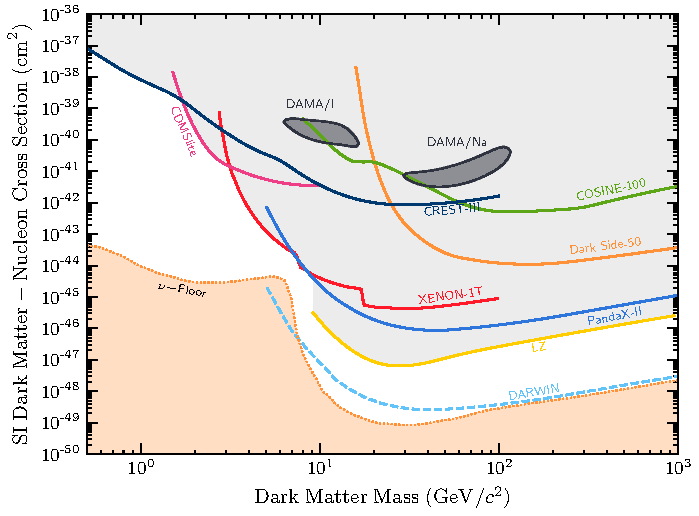
\includegraphics{img/chapter_1/DM_limits_SI.pdf}
    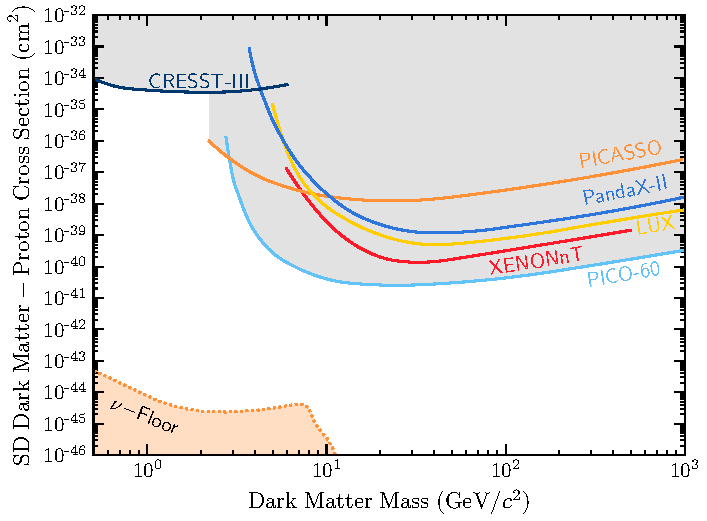
\includegraphics{img/chapter_1/DM_limits_SD_p.pdf}
    \caption{Current status of direct detection searches for dark matter. \textbf{Top:} Spin-independent dark matter-nucleon scattering. \textbf{Bottom:} Spin-dependent dark matter-proton scattering.}
    \label{fig:direct_detection_lims}
\end{figure}

The current leading constraints on the dark matter-nucleon scattering cross-section
are shown in Fig.~\ref{fig:direct_detection_lims}, with SI in the top panel and SD in the bottom.
The SI limits come from the liquid noble gas experiments (LZ~\cite{LZ:2022lsv_jul_FirstDarkMatter}, 
XENON-1T~\cite{XENON:2020gfr_mar_SearchCoherentElastic}, PandaX-II~\cite{PandaX-4T:2021bab_dec_DarkMatterSearch},
and DarkSide-50~\cite{DarkSide:2022dhx_mar_SearchDarkMatterNucleon}), solid-state cryogenic detectors (CRESST-III~\cite{CRESST:2019jnq_nov_FirstresultsCRESSTIII}, and CDMSlite~\cite{SuperCDMS:2023sql_jun_SearchLowmassDark}), 
and room temperature crystals (DAMA/LIBRA~\cite{Savage:2008er_CompatibilityDAMALIBRA}, and COSINE-100~\cite{COSINE-100:2021xqn_nov_StrongconstraintsCOSINE100}). 

The SD experiments require their targets to carry non-zero spin for the dark matter to couple to. 
$\ce{^{19}F}$ is the favourable choice proton scattering, as it has an unpaired proton giving it its overall spin.
The leading constraints come from superheated liquid experiments such as the PICO-60~\cite{PICO:2019vsc_jul_Darkmattersearch} as well as PICASSO~\cite*{Behnke:2016lsk_apr_FinalResultsPICASSO}
In terms of the SD proton scattering shown in Fig~\ref{fig:direct_detection_lims},
These interations are also searched for by many of the same experiments in the SI case, with the inclusion of
LZ's predecessor LUX~\cite{LUX:2017ree_jun_LimitsspindependentWIMPnucleon}.

\commMV{neutrino floor}

\commMV{shortfalls: min thresholds, decreas sensitity to hogher masses}



%%%%%%%%%%%%%%%%%%%%%%%%%%%%%%%%%%%%%
%%%%%%%%%%%%%%%%%%%%%%%%%%%%%%%%%%%%%
\subsection{Indirect Detection}
%%%%%%%%%%%%%%%%%%%%%%%%%%%%%%%%%%%%%
%%%%%%%%%%%%%%%%%%%%%%%%%%%%%%%%%%%%%


It is this route that we will follow to explore dark matter EFTs.

%%%%%%%%%%%%%%%%%%%%%%%%%%%%%%%%%%%%%
%%%%%%%%%%%%%%%%%%%%%%%%%%%%%%%%%%%%%
%%%%%%%%%%%%%%%%%%%%%%%%%%%%%%%%%%%%%
\section{Compact Objects as Dark Matter Probes}
%%%%%%%%%%%%%%%%%%%%%%%%%%%%%%%%%%%%%
%%%%%%%%%%%%%%%%%%%%%%%%%%%%%%%%%%%%%
%%%%%%%%%%%%%%%%%%%%%%%%%%%%%%%%%%%%%


Compact objects, namely Neutron Stars and White Dwarfs, offer a unique
laboratory for studying dark matter interactions. Their extreme environments
offer many benefits in comparison to direct detection experiments. 
These include:

\begin{itemize}
\item \textbf{Gravitational focusing of the DM flux.} In the NS case, the 
infalling DM will be boosted to semi-relativistic velocities ($\sim 0.2 - 0.7 c$
depending on the NS mass).
\item 
\end{itemize}


\begin{figure}
    \centering
    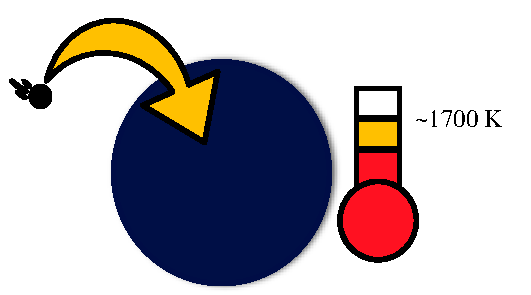
\includegraphics[width=0.45\textwidth]{img/chapter_1/kin_heat_NS.pdf}
    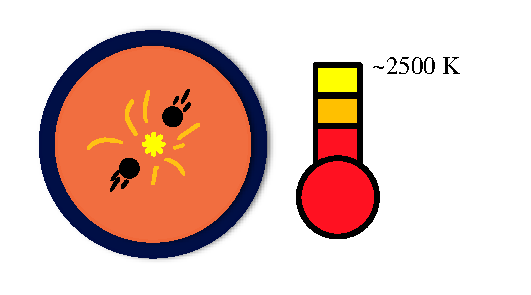
\includegraphics[width=0.45\textwidth]{img/chapter_1/ann_heat_NS.pdf}
    \caption{Illustration of DM-induced heating of compact objects. \textbf{Left:} kinetic heating due to DM scattering, raising the temperature to $\sim 1700 \K$. \textbf{Right:} further annihilation heating adding an additional $\sim 800\K$.}
    \label{fig:cartoon_NS_heat}
\end{figure}





We will study each operator in isolation, i.e. consider a Lagrangian that contains only one of the operators, rather than a linear superposition of multiple. This way, we can analyse specific types of interactions independently, allowing us to take as model-independent an approach to phenomenology as possible. 